\documentclass[a4paper, 12.5pt]{scrartcl}
\usepackage{german}
\usepackage[utf8]{inputenc}
\usepackage{graphicx}
\usepackage{amsmath}
\graphicspath{{./Figures/}}
\usepackage{hyperref}


\begin{document}


\begin{titlepage}
\author{Justin Sprenger (s0556255), 
Kai Thummerer (s0545266)} 
\title{- Bus bunching -\\
Datenimport, Verarbeitung und Darstellung von reellen Daten} 
\date{\today} 
\maketitle
\end{titlepage}

\tableofcontents
\newpage
\section{Einleitung}
\subsection{Problem- und Aufgabenstellung}
Ein bekanntes Problem im öffentlichem Verkehr ist das Bus bunching. Das bedeutet, dass der zeitlich geplante Verkehrsfluss aus dem Takt gerät und es somit zu Zeitverzögerungen und veränderten An- und Abfahrten kommt. Um diesem Problem vorzubeugen wird eine Software entwickelt, welche dem Zweck dient die aktuelle Position der Fahrzeuge bzw. auch den Abstand der Fahrzeuge darstellt, woraufhin schnell erkannt werden kann wo es zu Problemen führen kann.
Das Programm wird hierbei auf aufgezeichnete Daten zugreifen.

\section{Grundlagen}
\subsection{BVG-Datenbank}
Zur Bewältigung der Belegarbeit wurde eine Datenbank (in Form einer Dumpfile) der BVG inklusive der dazugehörigen Dokumentation bereitgestellt. In der Datenbank sind alle wichtigen Informationen der einzelnen Busse und der Bus-Linien abgespeichert.

\subsection{JavaFX} 

Die JavaFx , eine Java-Spezifikation von Oracle ist Bestandteil sämtlicher Java Plattformen. Beispielsweise JRE (Java SE Runtime Environment) und des JDK (Java Development Kit). Sie enthält Klassen und Interfaces, geschrieben in Java Code.
JavaFx löste die veralteten GUI-Toolkits AWT und Swing ab.
Mit dieser wird die Anfertigung , sowie Verteilung von multimedialen, interaktiven Inhalten und GUI’s (grafischen Benutzeroberflächen) vereinfacht.\\

\begin{figure}[h]
	\centering
	\includegraphics[scale=0.6]{javafx.png}
	\caption{JavaFx Architektur}
	\label{img:JavaFX}
\end{figure}
\newpage

\subsection{JDBC-API}
Die Java Database Connectivity steht für Java Datenverbindungsfähigkeit. Seit 1996 fungiert diese API  als Standard einer unabhängigen Schnittstelle zwischen der Programmiersprache Java zu relationalen Datenbanken differierender Hersteller.\\

JDBC übermittelt SQL-Anfragen zwischen der Java Anwendung und der Datenbank und gibt deren Ergebnisse, sofern vorhanden zurück.\\

Für jede spezifische DB ist ein spezieller JDBC Treiber erforderlich, der meist vom Anbieter des DB-Systems zur Verfügung gestellt wird.\\

JDBC Treiber unterteilen sich in 4 Kategorien :

\begin{itemize}
	\item Typ 1- JDBC-ODBC Bridge Driver
	\item Typ 2- Native-API Partly-Java Driver
	\item Typ 3- Net-Protocol All-Java Driver 
	\item Typ 4- Native-Protocol All-Java Driver 
\end{itemize}
\\
\begin{figure}[h]
	\centering
	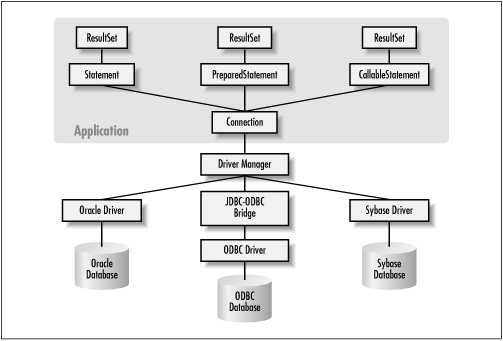
\includegraphics[scale=0.6]{jsp.png}
	\caption{JDBC API}
	\label{img:JDBC}
\end{figure}
\newpage


\section{Erstellen der Anwendung}

\subsection{MySQL-Import einer Oracle Dumpfile}

Mit Hilfe eines Dumpfile-Konverters ist es möglich die bereits bestehenden Oracle-Dumpfiles in MySQL-Dumpfiles zu konvertieren. Durch die Verwendung der kostenlosen Version des Konverters enthalten die Dumpfiles der Datenbanken nur noch 50 Einträge pro Tabelle. 
Die umgewandelten Dumpfiles können nun in MySQL-Datenbanken importiert werden.

\begin{figure}[h]
	\centering
	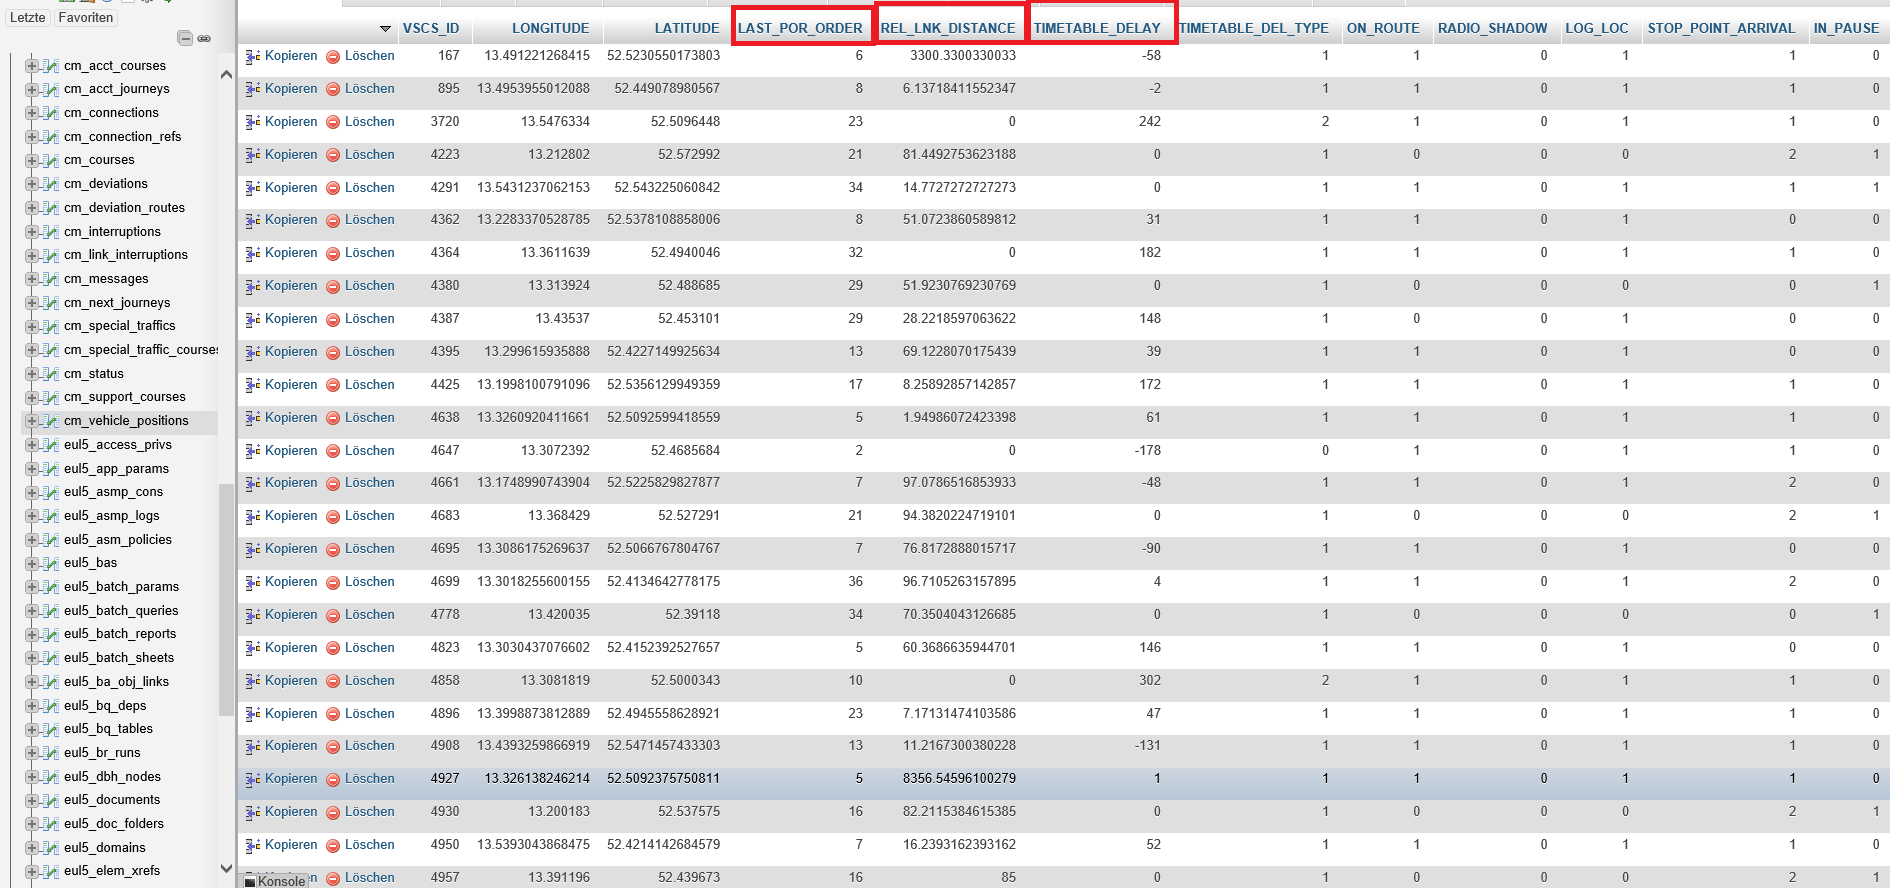
\includegraphics[scale=0.4]{Datenbank.png}
	\caption{Übersicht einer relevanten Tabelle}
	\label{img:grafik-DB}
\end{figure}

\subsection{Analyse der Datensätze aus der Dumpfile}
Bei der Formulierung der Abfragen gab es einige Probleme mit der Identifizierung der wichtigen Attribute der Tabellen. Einige der Attribute waren zwar in der Dokumentation der Datenbank enthalten, jedoch waren viele der relevanten nicht beschrieben. 
\\Die für die Abfragen relevanten Tabellen lauten :

\begin{itemize} 
\item Lines
\item Links
\item Points\_On\_Route
\item Network\_Points
\item Routes
\item Courses\_On\_Journey
\item cm\_vehicle\_positions
\item cm\_acct\_journey
\end{itemize}\\

Durch das importieren der Dumpfile in MySQL wurde die Konsistenz der Struktur bzw. die Beziehungen zwischen/in den Tabellen aufgehoben(Primär/Fremd-Schlüssel).
\\
Dadurch haben sich massive Probleme bei der Gestaltung der Abfragen ergeben.\newline
\label{sec:jump}
\newline Die Abfragen um den aktuellen Bus zu ermitteln(mit Beschreibung) lauten wie folgt:

\begin{small}
\\ 
\\ // Gibt die LDI-ID zurück, welche dazu dient die Routennummer und somit die Bushaltestellen-ID zu ermitteln
\\ 
\\ SELECT LDI\_ID
\\ FROM Lines
\\ WHERE NO like 192
\\ 
\\ // Gibt die Routennummer aus
\\ 
\\ SELECT ROU\_NO
\\ FROM Points\_On\_Route
\\ WHERE LDI\_ID like 10606661 
\\ 
\\ // Ermittelt aus den gelieferten Routennummern, die ID der Route, welche der Richtung entspricht
\\ 
\\ SELECT NO
\\ FROM ROUTES
\\ WHERE DIRECTION like ‘variable Richtung’ and NO like 118
\\ 
\\ // Liefert die Bushaltestellen-ID
\\ 
\\ SELECT NP\_ID
\\ FROM Points\_On\_Route
\\ WHERE LDI\_ID like 10606661 and ROU\_NO like 118
\\ 
\\ // Ermittelt anhand der Bushaltestellen-ID und der Haltestelle die Busnummer
\\ 
\\ SELECT VSCS\_ID
\\ FROM NETWORK\_POINTS
\\ WHERE ID like 3564322920 and Name like 'U Osloer Str.'
\\ 
\\ // Gibt die Zeitabweichung und die aktuelle Position in der Reihenfolge des Busses aus
\\ 
\\ SELECT TIMETABLE\_DELAY, LAST\_POR\_ORDER
\\ FROM CM\_VEHICLE\_POSITIONS
\\ WHERE VSCS\_ID Like '167'
\end{small}

\subsection{Implementieren der Hauptanwendung}
Zur Gestaltung der Anwendung wurde auf die JavaFX Api zurrückgegriffen. 
In der Grafischen Oberfläche hat der Nutzer die Möglichkeit die Buslinie anhand der Nummer, 
die Haltestelle und die Richtung anzugeben. Durch Klick auf den Button Start wird das Ergebnis in einer Tableview ausgegeben. In der TableView enthalten sind folgende Informationen:
Busliniennummer, aktuelle Haltestelle, Zeitabstand des Busses zur aktuellen Haltestelle.\\

\begin{figure}[h]
	\centering
	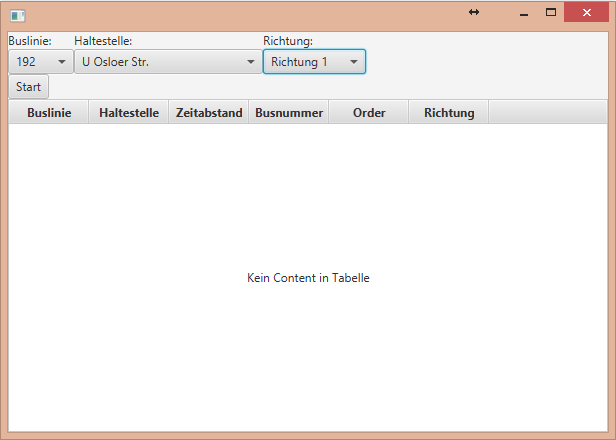
\includegraphics[scale=0.6]{Hauptanwendung.png}
	\caption{Hauptanwendung}
	\label{img:Hauptanwendung}
\end{figure}
\newpage

\subsection{Implementieren einer Datenbank-Schnittstelle}
Um eine Verbindung mit der Datenbank herstellen zu können wurde die JDBC-API verwendet. In dem Programm wurde eine Datenbank Klasse erstellt, welche diese Schnittstelle importiert und in welcher die SQL-Abfragen deklariert sind.\\

\begin{figure}[h]
	\centering
	\includegraphics[scale=0.55]{jdbc-database-example.png}
	\caption{JDBC DB Example}
	\label{img:JDBC}
\end{figure}

\subsection{Berechnung der Position der einzelnen Busse(Zeitabstand)}
Die Abstände müssen nicht direkt berechnet werden. in der Tabelle cm\_vehicle\_positions existiert die Spalte timedelay, welche die Verspätungen der einzelnen Busse zur nächsten Haltestelle in Sekunden angibt. Durch eine Abfrage, welche die ID des nächsten/vorherigen Busses ausgibt, kann der zeitliche Abstand zwischen dem Bus und der nachfolgenden und vorangegangenen Haltestelle ermittelt werden. Die Zeiten müssen gegebenenfalls zusammen addiert werden. Dies ist in diesem Fall jedoch nicht erforderlich, da jeweils nur ein Bus vorher und nachher ausgegeben wird.

\section{Ergebnis}
Aufgrund des Fehlerhaften Datenbank Imports in MySQL war es 
nicht möglich geschachtelte Abfragen zu formulieren. Aufgrund von unvollständigen Datensätzen ergeben sich aus den zusammenhängenden/passenden Abfragen keine vollständigen Resultate.

In dieser Anwendung musste aus gegebenen Umständen nicht zusammenhänge Datensätze verarbeitet werden.

Mittels einer funktionsfähigen Datenbank würden die im Anhang gezeigten SQL-Abfragen vermutlich zusammenhängende Ausgaben liefern.
\newpage

\section{Literaturverzeichnis}
\begin{thebibliography}{1}

  \bibitem{JavaFX} Christian Ullenboom {\em Java ist auch eine Insel (Auflage 12)} 2016.

\bibitem{JavaFX Overview (Release 8)}JavaFX Overview (Release 8) {\em https://docs.oracle.com/javase/8/javafx/get-started-tutorial/jfx-overview.htm\#JFXST784}

\bibitem{Java JDBC API}Java JDBC API {\em https://docs.oracle.com/javase/8/docs/technotes/guides/jdbc/}

\bibitem{Java SE Technologies}Java SE Technologies {\em http://www.oracle.com/technetwork/java/javase/jdbc/index.html}

\bibitem{JavaFX Tutorial}JAXenter 6 März 2017 {\em https://jaxenter.de/java-tutorial-javafx-53878}

\bibitem{Java Servlet Programming}Java Servlet Programming {\em https://docstore.mik.ua/orelly/java-ent/servlet/ch09\_02.htm}

\bibitem{Oracle Java Documentation}Oracle Java Documentation {\em https://docs.oracle.com/javase/8/docs/technotes/guides/jdbc/}

\bibitem{ora 2 MySQL}Ora2SQL Converter{\em https://www.convert-in.com/ord2sql.htm}

\end{thebibliography}

\section{Anhang}

\subsection{Alle ausgearbeiteten SQL-Abfragen}
\\
\begin{small}
\textbf{----- Aktueller Bus -----}
\\ \\
\hyperref[sec:jump]{siehe Punkt 3.2 - Analyse der Datensätze aus der Dumpfile}
\newline 
\\ \textbf{----- Nachfolgender Bus -----}
\newline 
\newline SELECT NP\_ID\_TO
\newline FROM LINKS
\newline WHERE NP\_ID like 3564322669
\newline 
\newline SELECT NP\_ID
\newline FROM POINTS\_ON\_ROUTE
\newline WHERE LDI\_ID like 10606661 and ROU\_NO like 118
\newline 
\newline SELECT ID
\newline FROM NETWORK\_POINTS
\newline WHERE ID like 3564322920 and Name like 'U Osloer Str.' 
\newline 
\newline SELECT VSCS\_ID
\newline FROM NETWORK\_POINTS
\newline WHERE ID like 3564322920 and Name like 'U Osloer Str.'
\newline 
\newline SELECT TIMETABLE\_DELAY, LAST\_POR\_ORDER
\newline FROM CM\_VEHICLE\_POSITIONS
\newline WHERE VSCS\_ID Like '167'
\newline 
\\ \textbf{----- Voriger Bus -----}
\newline 
\newline SELECT NP\_ID
\newline FROM LINKS
\newline WHERE NP\_ID\_TO like 3564322669 and ID like 728
\newline 
\newline SELECT NP\_ID
\newline FROM POINTS\_ON\_ROUTE
\newline WHERE LDI\_ID like 10606661 and ROU\_NO like 118
\newline 
\newline SELECT ID
\newline FROM NETWORK\_POINTS
\newline WHERE ID like 3564322920 and Name like 'U Osloer Str.' 
\newline 
\newline SELECT VSCS\_ID
\newline FROM NETWORK\_POINTS
\newline WHERE ID like 3564322920 and Name like 'U Osloer Str.'
\newline 
\newline SELECT TIMETABLE\_DELAY, LAST\_POR\_ORDER
\newline FROM CM\_VEHICLE\_POSITIONS
\newline WHERE VSCS\_ID Like '167'
\newline 
\\ \textbf{----- Richtung -----}
\newline 
\newline SELECT REMARK
\newline FROM LINES
\newline WHERE NO like 255
\end{small}
\end{document}